	
\documentclass[a4paper,12pt]{article} 
\usepackage{amsmath, amssymb}
\usepackage{kotex}
\usepackage{graphicx}
\usepackage[figuresright]{rotating} 

\begin{document} 

\title{과제5 보고서}
\author{B211103 변준석}
\date{2017년 10월}
\maketitle

\newpage
\section{개요}
이번 과제의 메인 프로그램인 \textsl{hw5.cpp} 에서는 스택 자료구조를 이용한 Maze의 경로 찾기 프로그램을 구현하였다.

\section{문제 해결 방안}
\textsl{maze}문제의 해결을 위하여 이동 방향을 결정하는 구조체\textsl{offsets}와 현재 위치 및 이동 방향을 값으로 갖는 구조체\textsl{Items}를 설계하였다. 경로를 찾는 함수는 \textsl{Path}로 구현하였다.

\section{\textsl{최종 출력}}
\newpage
\begin{figure}[t]\vspace*{4pt} 
\centerline{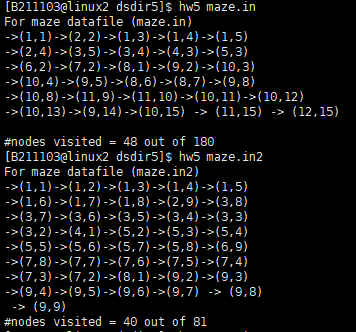
\includegraphics[width=1.0\columnwidth]{result}} 
\caption{matrixa.cpp의 Transpose 구현}\vspace*{-6pt} 
\label{figure:matrixa} 
\end{figure} 


 
\section{hw5의 간단한 설명}
모든 기능들이 정상작동함을 알 수 있다. \textsl{nodes visited}변수는 스태틱 변수이며 \textsl{mark}프로세스마다 1씩 증가하였다.
 

\newpage
\begin{figure}[t]\vspace*{4pt} 
\centerline{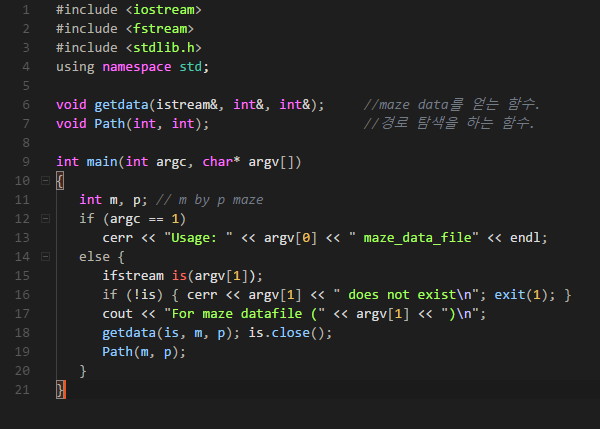
\includegraphics[width=1.0\columnwidth]{hw5cpp}} 
\caption{hw5.cpp}\vspace*{-6pt} 
\label{figure:hw5cpp} 
\end{figure} 

\begin{figure}[t]\vspace*{4pt} 
\centerline{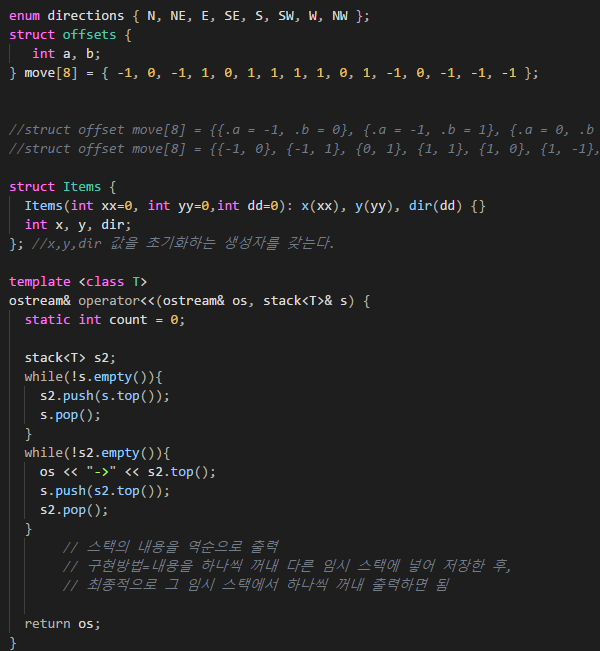
\includegraphics[width=1.0\columnwidth]{maze1}} 
\caption{offsets와 Items의 구조체}\vspace*{-6pt} 
\label{figure:matrixa_overload} 
\end{figure} 

\newpage
\begin{figure}[t]\vspace*{4pt} 
\centerline{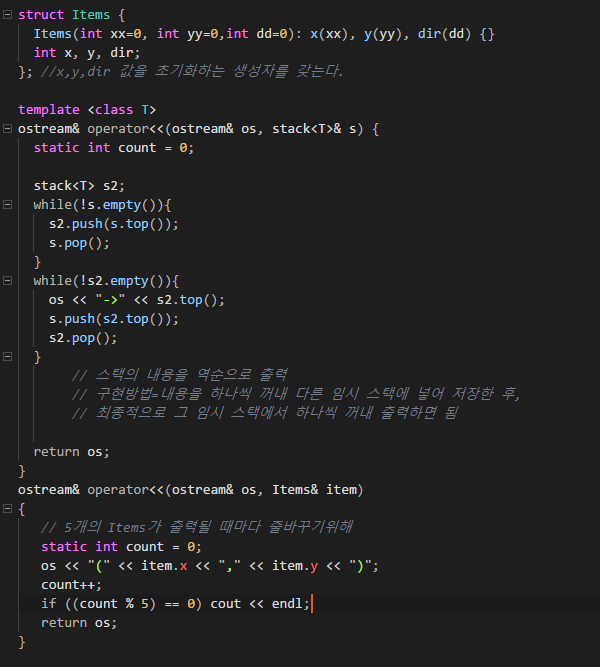
\includegraphics[width=1.0\columnwidth]{maze2}} 
\caption{출력을 위한 연산자 오버로딩}\vspace*{-6pt} 
\label{figure:matrixb} 
\end{figure} 

\begin{figure}[t]\vspace*{4pt} 
\centerline{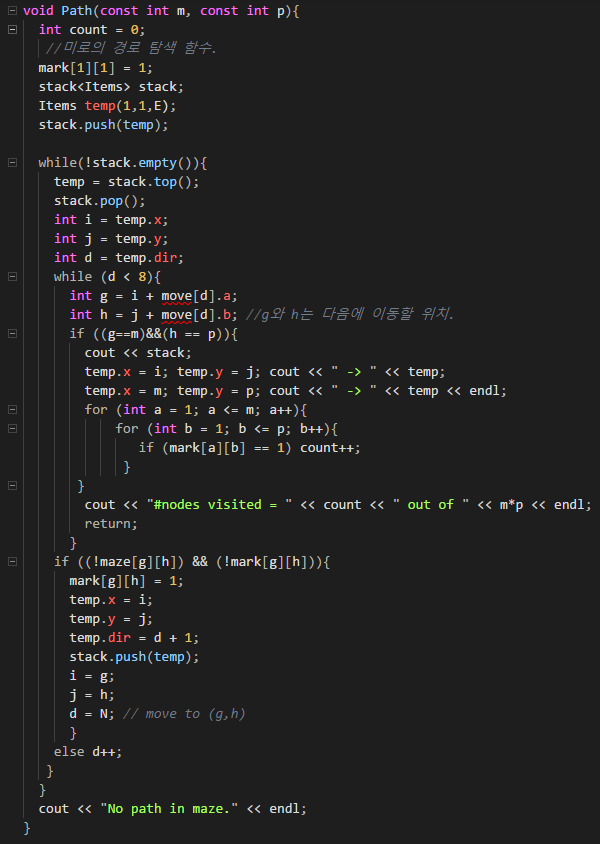
\includegraphics[width=1.0\columnwidth]{maze3}} 
\caption{경로찾기 함수}\vspace*{-6pt} 
\label{figure:matrixb_overload} 
\end{figure} 

\begin{figure}[t]\vspace*{4pt} 
    \centerline{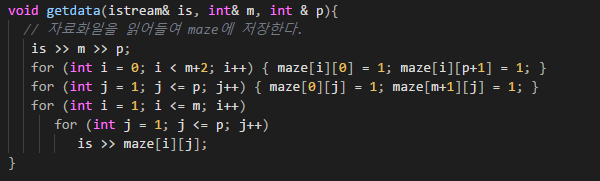
\includegraphics[width=1.0\columnwidth]{maze4}} 
    \caption{메이즈 데이터 받는 함수}\vspace*{-6pt} 
    \label{figure:matrixb_overload} 
    \end{figure} 
    
\end{document} 